\documentclass{beamer}

\usepackage[utf8]{inputenc}
\usepackage[square]{natbib}
\usepackage{ragged2e}

\renewcommand{\bibsection}{\subsubsection*{\bibname }}

\setbeamertemplate{caption}[numbered]
\renewcommand{\figurename}{Figura}
\renewcommand{\tablename}{Tabela}

\usetheme{Madrid}
\usecolortheme{default}
\useoutertheme{miniframes}

%------------------------------------------------------------
%This block of code defines the information to appear in the
%Title page
\title[] % (optional)
{Predição da Geração de Energia Utilizando Dados Climáticos}

\author[Vitor~Oliveira~Ropke] % (optional)
{
    Vitor~Oliveira~Ropke
}

\institute[] % (optional)
{
    
\includegraphics[height=1.5cm]{brasao-uern.png}
    \hspace{3cm}
    
\includegraphics[height=1.5cm]{logo-ppgcc.png}
    \hspace{3cm}
    
\includegraphics[height=1.5cm]{brasao-ufersa.eps}
}

\date[Dezembro de 2024] % (optional)
{Dezembro de 2024}

%End of title page configuration block
%------------------------------------------------------------

\begin{document}

%Hide the navigation buttons
\beamertemplatenavigationsymbolsempty

%The next statement creates the title page
\frame{\titlepage}

%---------------------------------------------------------


\section{Introdução}


%---------------------------------------------------------
\begin{frame}
\frametitle{Mudanças Climáticas}
\begin{itemize}
    \item Alteração dos padrões climáticos
    \item Anomalia de precipitação, chuva e radiação solar
    \item Impacta o setor elétrico dos países
\end{itemize}
\end{frame}
%---------------------------------------------------------


%---------------------------------------------------------
\begin{frame}
\frametitle{Sistema Interligado Nacional (SIN)}
\begin{itemize}
    \item Centraliza geração e distribuição de energia
    \item Possui suas vantagens e desvantagens
\end{itemize}
\end{frame}
%---------------------------------------------------------


%---------------------------------------------------------
\begin{frame}
\frametitle{Sistema Interligado Nacional (SIN)}
\begin{figure}
    \centering
    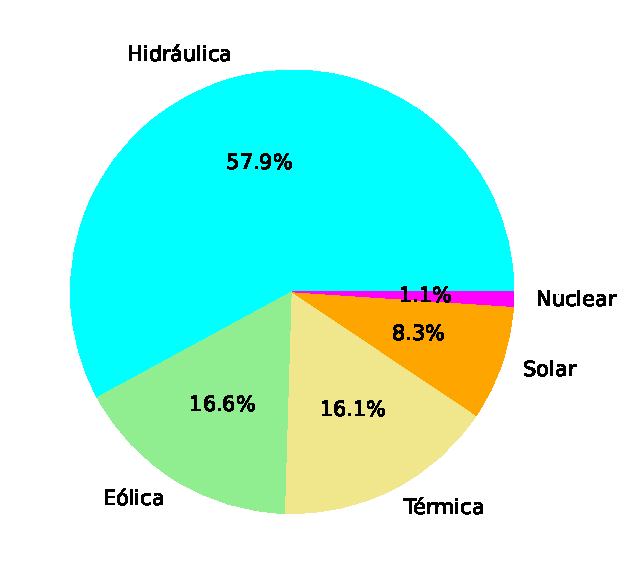
\includegraphics[width=0.5\linewidth]{matriz-energetica.pdf}
    \caption{Matriz Energética Brasileira no Dia 30 de Novembro de 2024}
\end{figure}
\end{frame}
%---------------------------------------------------------


%---------------------------------------------------------
\begin{frame}
\frametitle{Objetivo}
Identificar possíveis momentos críticos de geração de energia.
\end{frame}
%---------------------------------------------------------


\section{Metodologia}


%---------------------------------------------------------
\begin{frame}
\frametitle{Estratégia}

\begin{columns}
    \column{0.48\textwidth}
    
    \begin{block}{1ª etapa}
    Predição dos elementos climáticos usando o Prophet.
    \vspace{5.4mm}
    \begin{itemize}
        \item Chuva
        \vspace{5.4mm}
        \item Sol
        \vspace{5.4mm}
        \item Vento
    \end{itemize}
    \end{block}

    \column{0.48\textwidth}
    
    \begin{block}{2ª etapa}
    Predição da geração e do consumo de energia usando o NeuralProphet.
    \begin{itemize}
        \item Geração hidráulica -- Chuva
        \item Geração fotovoltaica -- Sol
        \item Geração eólica -- Vento
        \item Geração térmica
        \item Consumo
    \end{itemize}
    \end{block}
\end{columns}

\end{frame}
%---------------------------------------------------------


%---------------------------------------------------------
\begin{frame}
\frametitle{Coleta de Dados}
3 datasets
\begin{itemize}
    \item Elementos climáticos
    \item Capacidade de geração
    \item Geração e consumo
\end{itemize}
\end{frame}
%---------------------------------------------------------


%---------------------------------------------------------
\begin{frame}
\frametitle{Coleta de Dados - Elementos Climáticos}
\begin{itemize}
    \item \href{https://portal.inmet.gov.br/dadoshistoricos}{portal.inmet.gov.br/dadoshistoricos}
    \begin{columns}
        \column{0.5\textwidth}
        \begin{figure}
            \centering
            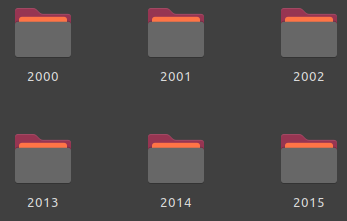
\includegraphics[width=0.7\linewidth]{pastas-inmet.png}
        \end{figure}
    
        \column{0.5\textwidth}

        \begin{figure}
            \centering
            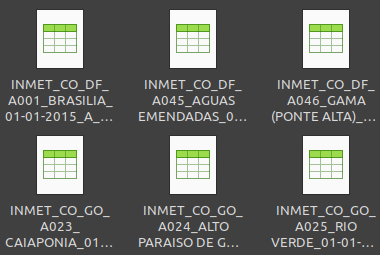
\includegraphics[width=0.7\linewidth]{estacoes-inmet.png}
        \end{figure}
    \end{columns}
    \item \href{https://bdmep.inmet.gov.br}{bdmep.inmet.gov.br}
    \begin{figure}
        \centering
        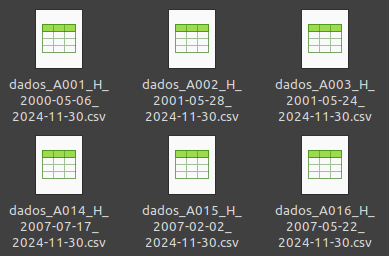
\includegraphics[width=0.4\linewidth]{estacoes-bdmep.png}
    \end{figure}
\end{itemize}
\end{frame}
%---------------------------------------------------------


%---------------------------------------------------------
\begin{frame}
\frametitle{Coleta de Dados - Elementos Climáticos}
\begin{itemize}
    \item Dados horários
    \item 19 colunas (\href{https://portal.inmet.gov.br/dadoshistoricos}{INMET DADOS HISTÓRICOS ANUAIS})
    \item 5 colunas (\href{https://bdmep.inmet.gov.br}{INMET::BDMEP})
    \begin{itemize}
        \item \texttt{Data Medicao}
        \item \texttt{Hora Medicao}
        \item \texttt{PRECIPITACAO TOTAL, HORARIO(mm)}
        \item \texttt{RADIACAO GLOBAL(Kj/m²)}
        \item \texttt{VENTO, VELOCIDADE HORARIA(m/s)}
    \end{itemize}
    \item 634 estações meteorológicas (\href{https://portal.inmet.gov.br/dadoshistoricos}{INMET DADOS HISTÓRICOS ANUAIS})
    \item 602 estações meteorológicas (\href{https://bdmep.inmet.gov.br}{INMET::BDMEP})
\end{itemize}
\end{frame}
%---------------------------------------------------------


%---------------------------------------------------------
\begin{frame}
\frametitle{Coleta de Dados - Capacidade de Geração}
\begin{itemize}
    \item \href{https://dados.ons.org.br/dataset/capacidade-geracao}{dados.ons.org.br/dataset/capacidade-geracao}
    \item Dados diários
    \item 17 colunas (4 selecionadas)
    \begin{itemize}
        \item \texttt{nom\char`_tipousina}
        \item \texttt{dat\char`_entradaoperacao}
        \item \texttt{dat\char`_desativacao}
        \item \texttt{val\char`_potenciaefetiva}
    \end{itemize}
    \item 1 arquivo
    \item 5.201 linhas
\end{itemize}
\end{frame}
%---------------------------------------------------------


%---------------------------------------------------------
\begin{frame}
\frametitle{Coleta de Dados - Geração e Consumo}
\begin{itemize}
    \item \href{https://dados.ons.org.br/dataset/balanco-energia-subsistema}{dados.ons.org.br/dataset/balanco-energia-subsistema}
    \begin{figure}
        \centering
        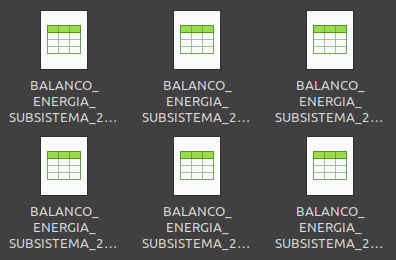
\includegraphics[width=0.6\linewidth]{arquivos-geracao-consumo.png}
    \end{figure}
\end{itemize}
\end{frame}
%---------------------------------------------------------


%---------------------------------------------------------
\begin{frame}
\frametitle{Coleta de Dados - Geração e Consumo}
\begin{itemize}
    \item Dados horários
    \item 9 colunas (7 selecionadas)
    \begin{itemize}
        \item \texttt{nom\char`_subsistema}
        \item \texttt{din\char`_instante}
        \item \texttt{val\char`_gerhidraulica}
        \item \texttt{val\char`_gertermica}
        \item \texttt{val\char`_gereolica}
        \item \texttt{val\char`_gersolar}
        \item \texttt{val\char`_carga}
    \end{itemize}
    \item 25 arquivos
    \item 43.916 linhas, cada
\end{itemize}
\end{frame}
%---------------------------------------------------------


%---------------------------------------------------------
\begin{frame}
\frametitle{Processamento de Dados - Elementos Climáticos}
\begin{itemize}
    \item Seleção de estações meteorológicas com no mínimo 30\% de dados válidos
    \item Seleção de estações meteorológicas com no mínimo 2 anos (730 dias) de dados
    \item 582 estações meteorológicas com predição feita
    \item Dados horários reamostrados para dados diários, fazendo a média dos valores horários
    \item Dados diários de 6 de Maio de 2000 até 30 de Novembro de 2024
\end{itemize}
\end{frame}
%---------------------------------------------------------


%---------------------------------------------------------
\begin{frame}
\frametitle{Processamento de Dados - Elementos Climáticos}
\begin{table}[ht]
    \centering
    \begin{tabular}{l c c c}
        \hline
        data & chuva & sol & vento \\
        \hline
        2000-05-06 & 0.01837 & 1278.09386 & 2.35468 \\
        2000-05-07 & 0.02028 & 1295.12063 & 2.33444 \\
        2000-05-08 & 0.01546 & 1269.16514 & 2.33220 \\
        2000-05-09 & 0.00931 & 1288.86107 & 2.33925 \\
        \hline
    \end{tabular}
    \caption{Amostra dos Dados Climáticos}
\end{table}
\end{frame}
%---------------------------------------------------------


%---------------------------------------------------------
\begin{frame}
\frametitle{Processamento de Dados - Capacidade de Geração}
\begin{itemize}
    \item Dados inicialmente classificados por usina
    \item Cada usina possui data de início de operação e pode ter data de fim de operação
    \item Iteração diária de 6 de Maio de 2000 até 30 de Novembro de 2024
    \item Soma da potência de cada usina de acordo com o tipo e a data de início e fim de operação
    \item Resulta em uma tabela com a capacidade de geração diária de cada tipo de energia
\end{itemize}
\end{frame}
%---------------------------------------------------------


%---------------------------------------------------------
\begin{frame}
\frametitle{Processamento de Dados - Capacidade de Geração}
\begin{itemize}
    \item 7 colunas
    \begin{itemize}
        \item \texttt{data}
        \item \texttt{potencia\char`_total}
        \item \texttt{potencia\char`_hidraulica}
        \item \texttt{potencia\char`_termica}
        \item \texttt{potencia\char`_eolica}
        \item \texttt{potencia\char`_solar}
        \item \texttt{potencia\char`_nuclear}
    \end{itemize}
\end{itemize}
\end{frame}
%---------------------------------------------------------


%---------------------------------------------------------
\begin{frame}
\frametitle{Processamento de Dados - Capacidade de Geração}
\begin{table}[ht]
    \centering
    \resizebox{\columnwidth}{!}{%
        \begin{tabular}{l c c c c c r}
            \hline
            data & potencia\_total & potencia\_hidraulica & potencia\_termica & potencia\_eolica & potencia\_solar & potencia\_nuclear \\
            \hline
            2000-05-06 & 68682.88600 & 63756.91999 & 4285.96599 & 0.0 & 0.0 & 640.0 \\
            2000-05-07 & 68682.88600 & 63756.91999 & 4285.96599 & 0.0 & 0.0 & 640.0 \\
            2000-05-08 & 68682.88600 & 63756.91999 & 4285.96599 & 0.0 & 0.0 & 640.0 \\
            2000-05-09 & 68682.88600 & 63756.91999 & 4285.96599 & 0.0 & 0.0 & 640.0 \\
            \hline
        \end{tabular}%
    }
    \caption{Amostra dos Dados da Capacidade de Geração}
\end{table}
\end{frame}
%---------------------------------------------------------


%---------------------------------------------------------
\begin{frame}
\frametitle{Processamento de Dados - Geração e Consumo}
\begin{itemize}
    \item Seleção de linhas onde \texttt{SISTEMA INTERLIGADO NACIONAL} é o valor em \texttt{nom\char`_subsistema}
    \item Dados horários reamostrados para dados diários, fazendo a média dos valores horários
    \item Dados diários de 6 de Maio de 2000 até 30 de Novembro de 2024
\end{itemize}
\end{frame}
%---------------------------------------------------------


%---------------------------------------------------------
\begin{frame}
\frametitle{Processamento de Dados - Geração e Consumo}
\begin{table}[ht]
    \centering
    \resizebox{\columnwidth}{!}{%
        \begin{tabular}{l c c c c r}
            \hline
            data & val\_gerhidraulica & val\_gertermica & val\_gereolica & potencia\_gersolar & potencia\_carga \\
            \hline
            2000-05-06 & 37575.91666 & 1785.445833 & 0.0 & 0.0 & 39408.67916 \\
            2000-05-07 & 32997.02083 & 1706.8875 & 0.0 & 0.0 & 34751.125 \\
            2000-05-08 & 39447.27083 & 1825.325 & 0.0 & 0.0 & 41444.38333 \\
            2000-05-09 & 40412.70833 & 1786.9375 & 0.0 & 0.0 & 42356.49166 \\
            \hline
        \end{tabular}%
    }
    \caption{Amostra dos Dados de Geração e Consumo}
\end{table}
\end{frame}
%---------------------------------------------------------


\section{Resultados}


%---------------------------------------------------------
\begin{frame}
\frametitle{Predição dos Elementos Climáticos}
\begin{figure}
    \centering
    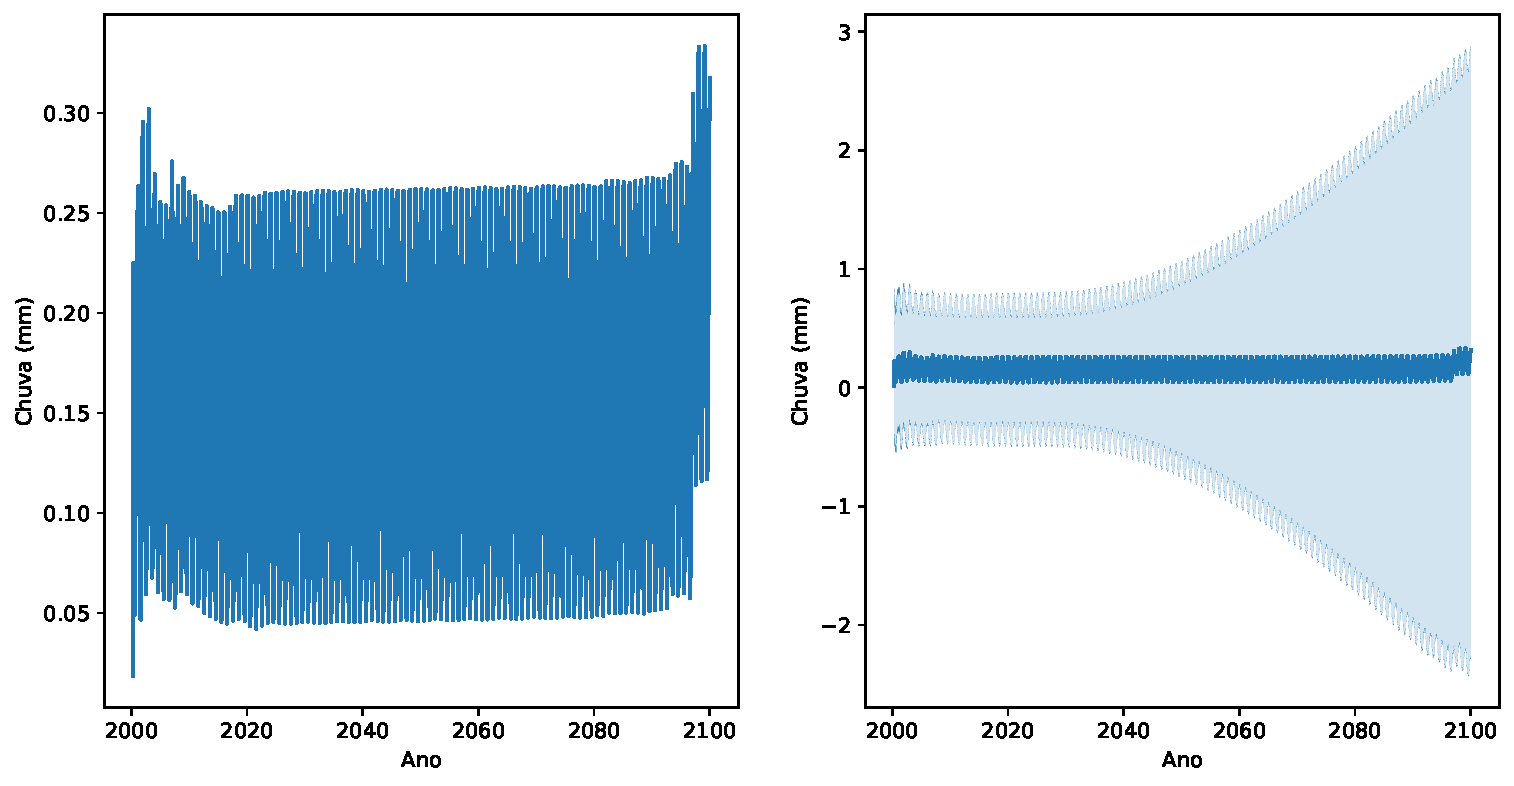
\includegraphics[width=0.9\linewidth]{chuva.pdf}
    \caption{Evolução da Chuva ao Longo dos Anos}
\end{figure}
\end{frame}
%---------------------------------------------------------


%---------------------------------------------------------
\begin{frame}
\frametitle{Predição dos Elementos Climáticos}
\begin{figure}
    \centering
    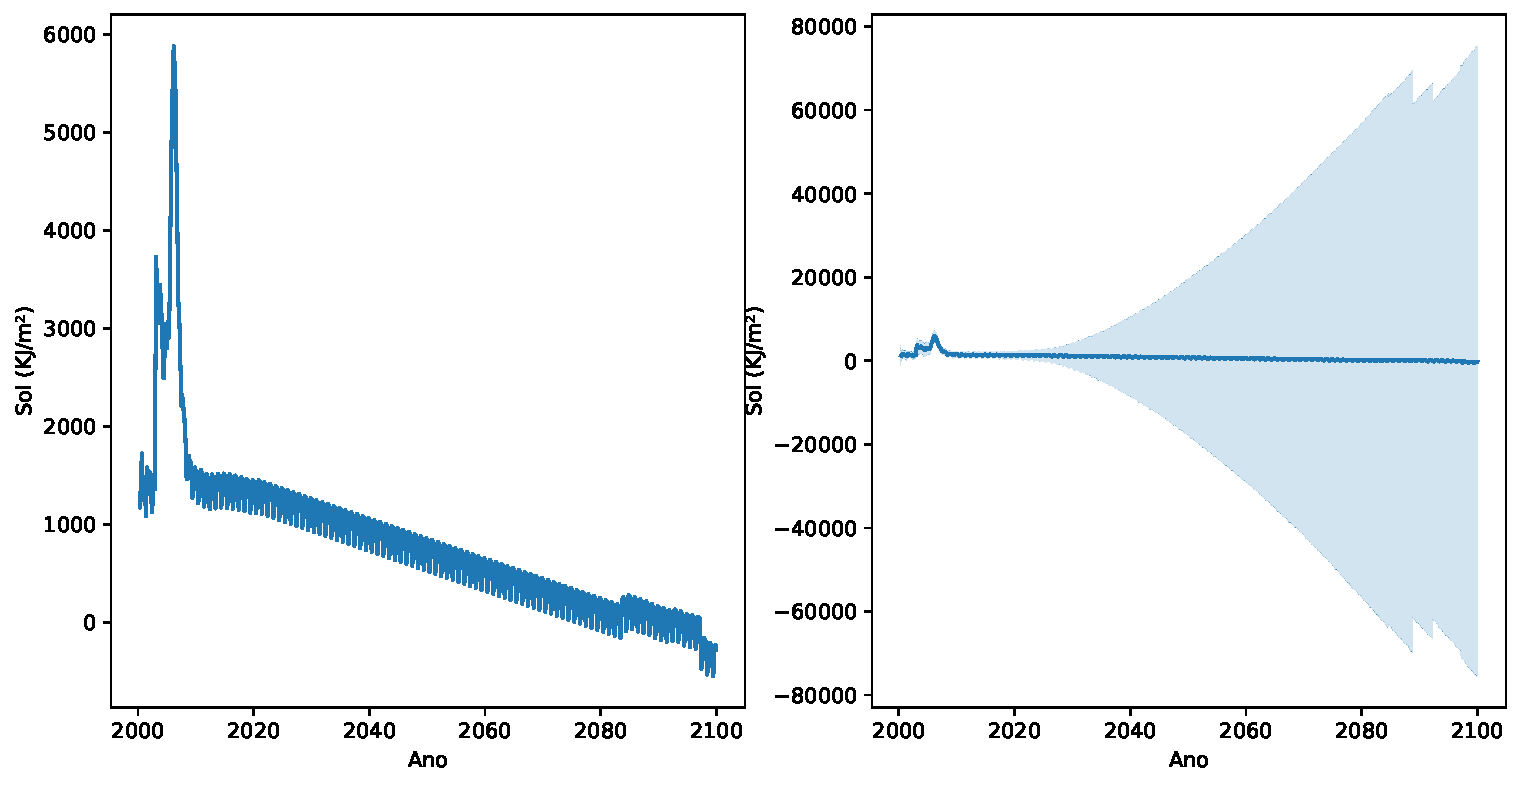
\includegraphics[width=0.9\linewidth]{sol.pdf}
    \caption{Evolução da Radiação Solar ao Longo dos Anos}
\end{figure}
\end{frame}
%---------------------------------------------------------


%---------------------------------------------------------
\begin{frame}
\frametitle{Predição dos Elementos Climáticos}
\begin{figure}
    \centering
    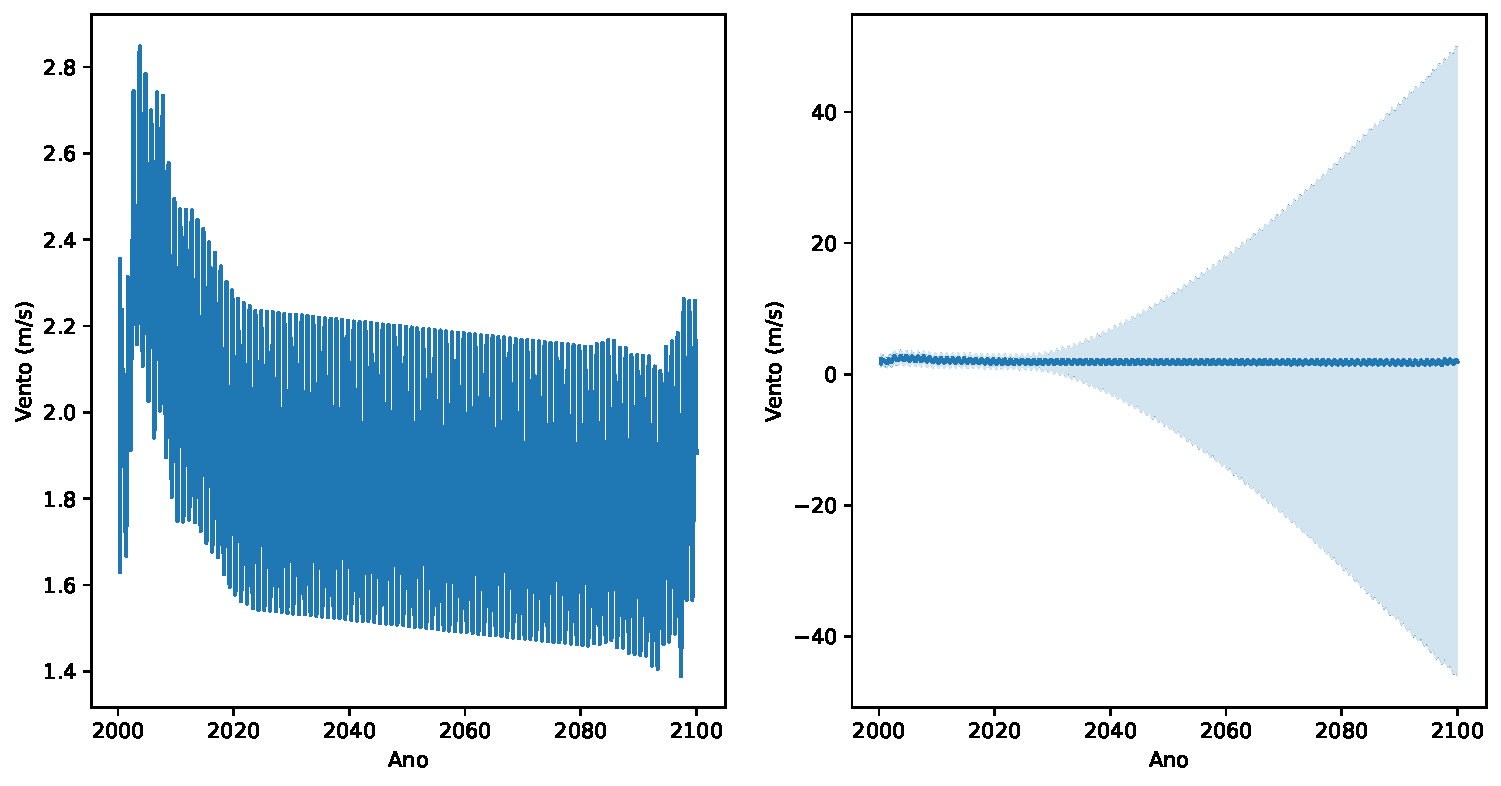
\includegraphics[width=0.9\linewidth]{vento.pdf}
    \caption{Evolução da Velocidade do Vento ao Longo dos Anos}
\end{figure}
\end{frame}
%---------------------------------------------------------


%---------------------------------------------------------
\begin{frame}
\frametitle{Capacidade de Geração}
\begin{figure}
    \centering
    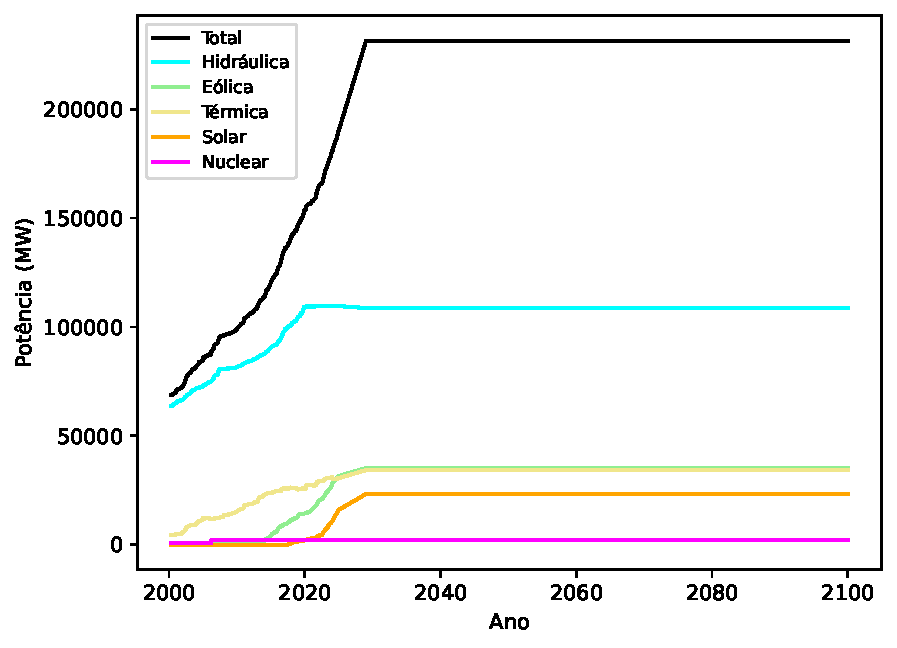
\includegraphics[width=0.6\linewidth]{capacidade-geracao.pdf}
    \caption{Evolução da Capacidade de Geração ao Longo dos Anos}
\end{figure}
\end{frame}
%---------------------------------------------------------


%---------------------------------------------------------
\begin{frame}
\frametitle{Geração e Consumo}
\begin{figure}
    \centering
    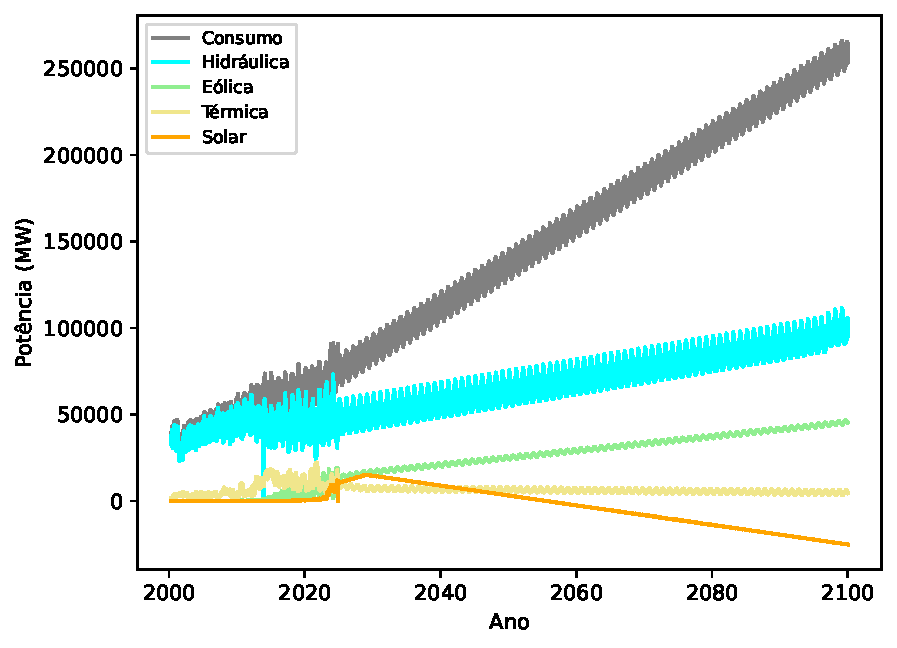
\includegraphics[width=0.6\linewidth]{geracao-consumo.pdf}
    \caption{Evolução da Geração e do Consumo ao Longo dos Anos}
\end{figure}
\end{frame}
%---------------------------------------------------------



%---------------------------------------------------------
\begin{frame}
\frametitle{Capacidade, Geração e Consumo}
\begin{figure}
    \centering
    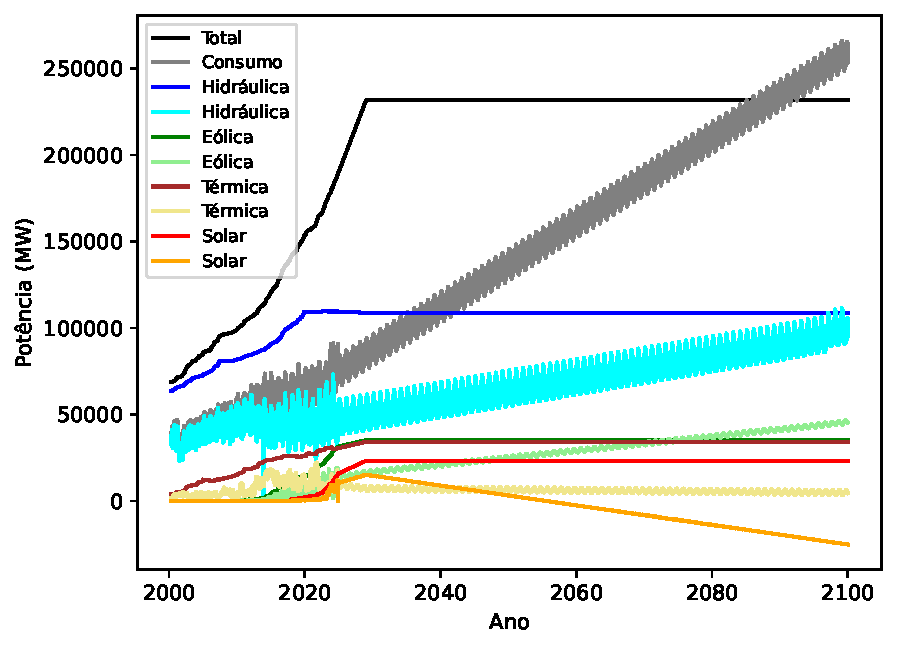
\includegraphics[width=0.6\linewidth]{capacidade-geracao-consumo.pdf}
    \caption{Comparação da Capacidade de Geração com a Geração e Consumo}
\end{figure}
\end{frame}
%---------------------------------------------------------


\section{Discussões}


%---------------------------------------------------------
\begin{frame}
\frametitle{Conclusões}
\begin{itemize}
    \item Prophet e NeuralProphet conseguem fazer as predições mesmo sem ajustar os parâmetros
    \item Resultados mostram que o consumo passa pela geração total por volta de 2080
\end{itemize}
\end{frame}
%---------------------------------------------------------


%---------------------------------------------------------
\begin{frame}[allowframebreaks]
\frametitle{Trabalhos Futuros}
\begin{itemize}
    \item Ajustar os parâmetros
    \item Diminuir a tolerância para valores nulos e zerados
    \item Considerar correlações entre os tipos de geração e os elementos climáticos
    \begin{itemize}
        \item Considerar efeitos da chuva sobre a geração solar e eólica
        \item Considerar efeitos do sol sobre a geração hidrelétrica e eólica
        \item Considerar efeitos do vento sobre a geração hidrelétrica e solar
    \end{itemize}
    \item Considerar a geolocalização das usinas e das estações meteorológicas
\end{itemize}
\end{frame}
%---------------------------------------------------------


\section*{}
\setcounter{section}{0}


%---------------------------------------------------------
\begin{frame}
\begin{center}
    \Huge ACABOU-SE!!!
\end{center}
\begin{figure}
    \centering
    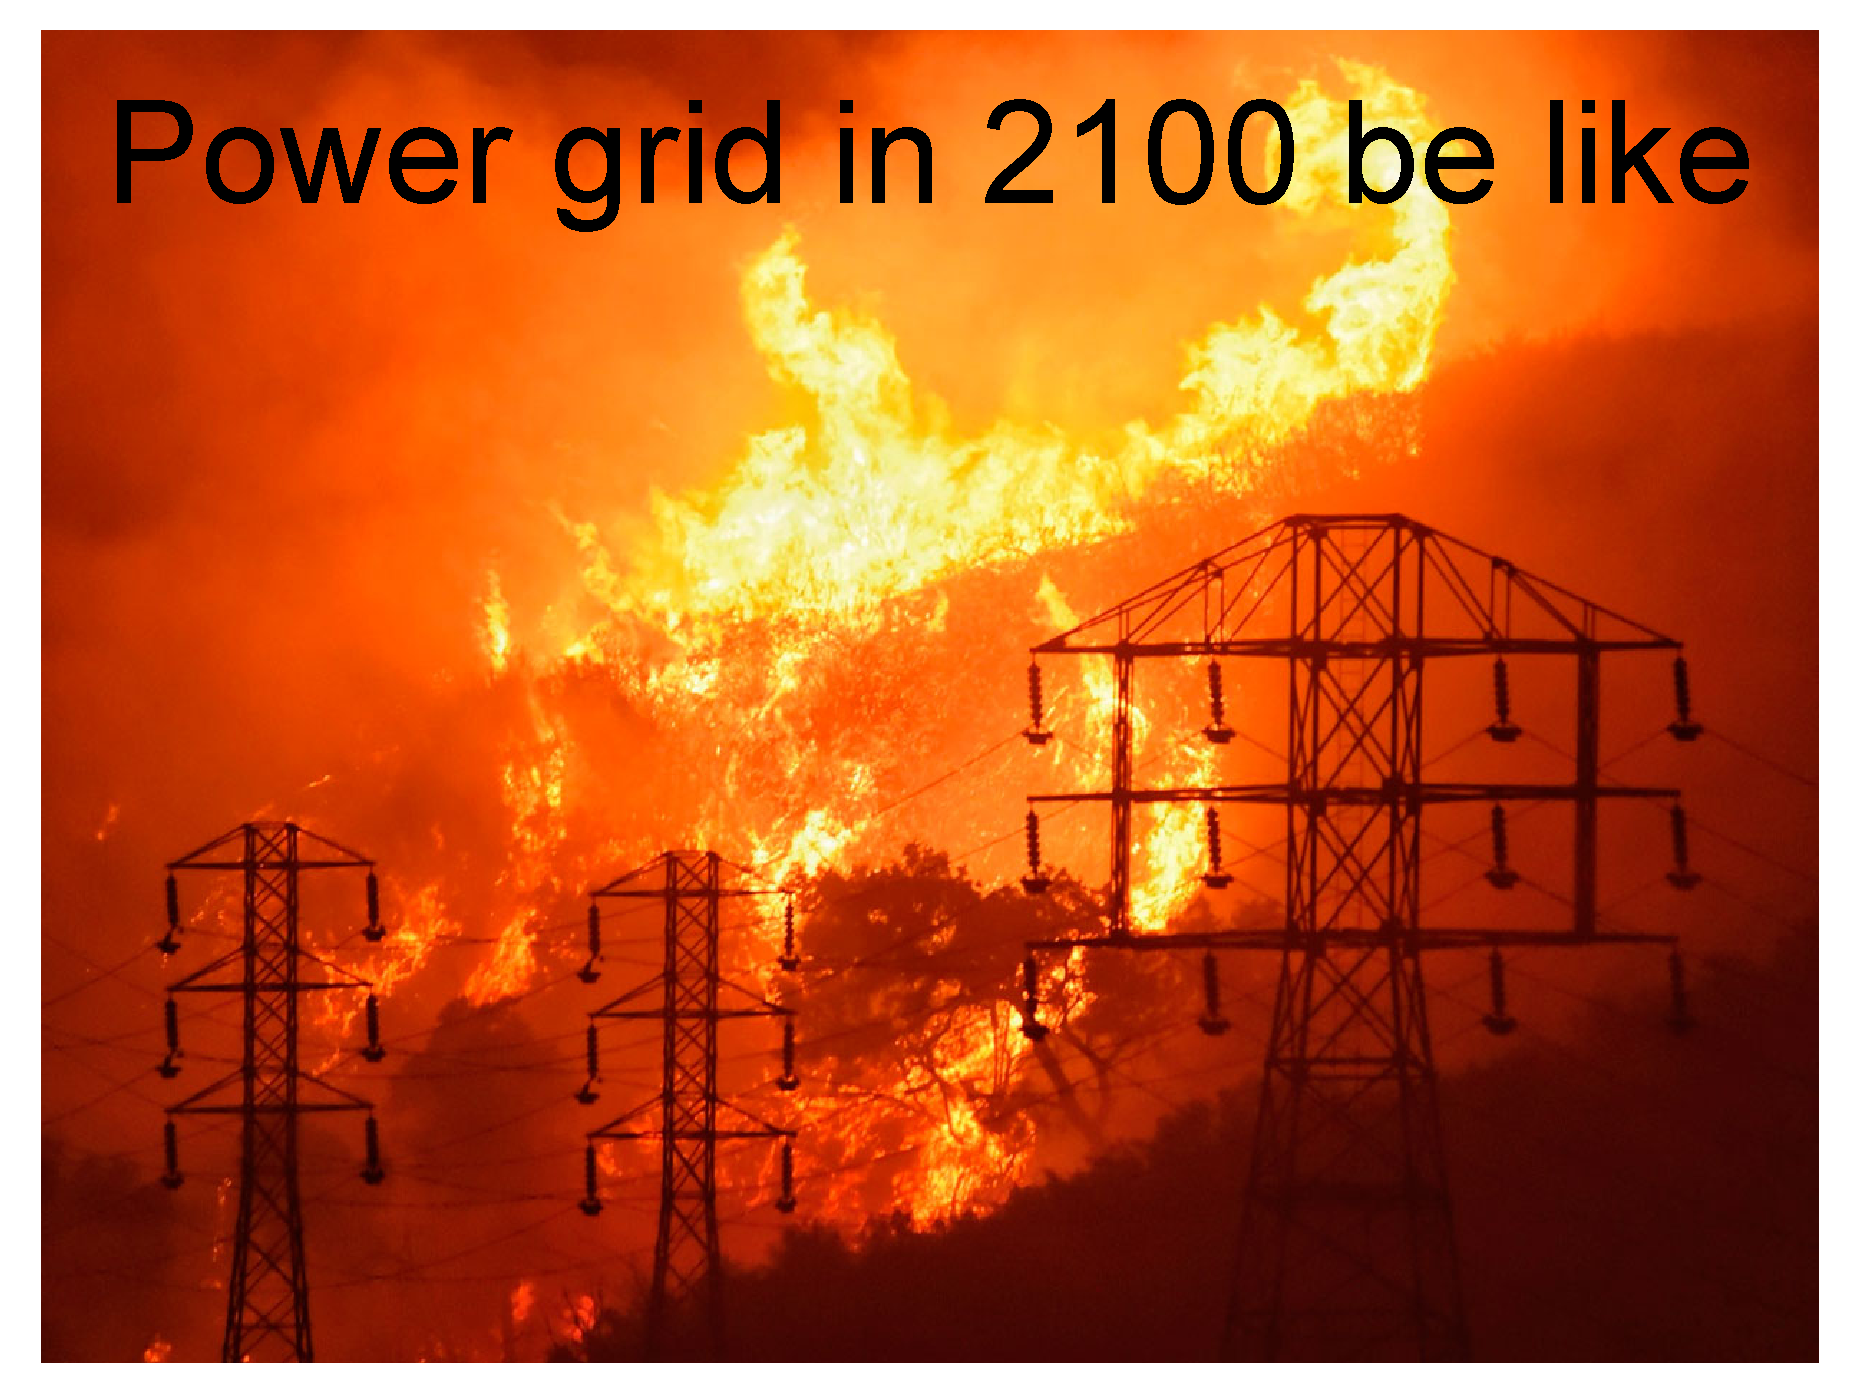
\includegraphics[width=0.7\linewidth]{power-grid-2100-be-like.pdf}
\end{figure}
\end{frame}
%---------------------------------------------------------


\end{document}
